\subsection{Removing strategy hints from unchanged problems}

\label{sec:prompt-hint-ablation}

We compare original and neutral prompts on \texttt{Python}, \texttt{MathIR}, and \texttt{PantryPlan} at Levels 2 and 3. Each of the six domain--level combinations uses 32 problems selected independently of model outputs from the 128-problem evaluation split. We sample eight responses per problem under each wording. The original wording uses the standard prompt. The neutral wording removes the \texttt{Python} nested-conditional example and suggestions to test small divisors or dispatch on listed values, the \texttt{MathIR} ordered algebraic-isolation suggestion, and the \texttt{PantryPlan} preference for ingredients high in energy and protein but low in sodium such as seeds or oats. \texttt{MathIR} changes ``those operations'' to ``the operations'' to preserve the instruction to return a menu ID. The problem instance, answer specification, executable verifier, and remaining format requirements are unchanged.

The paired effects are neutral minus original on empirical $P_8=\texttt{pass@8}$ and $D_8=\texttt{distinct@8}$, with $B_8=D_8-P_8$ as extra verified modes per problem. Incorrect, empty, and truncated outputs remain in their eight-draw groups; only verifier-accepted outputs contribute a verified key. Results use strict verification. A sensitivity analysis with normalized formatting preserves every strict success and canonical key and applies the same rules to both arms.

Intervals use 20,000 whole-problem bootstrap resamples, paired across arms and stratified by domain and level. Domain--level combinations receive equal weight in aggregate estimates. The intervals are pointwise 95\% percentile intervals without multiplicity adjustment. With 32 problems per domain and level, an interval crossing zero does not establish equivalence. A zero-width interval reflects zero variation in the observed bootstrap resamples, including identical paired $P_8$ outcomes, and does not establish population equivalence. Correct-pair collision and its certified-support uniform reference use the same correct-pair weights. Eight draws per prompt do not identify total unseen support.



We evaluate the initial Qwen2.5-0.5B-Instruct checkpoint and Level-2-trained Dr.GRPO and Re:Dr checkpoints. \texttt{Python} and \texttt{MathIR} use five matched training seeds; \texttt{PantryPlan} uses two. Level 3 tests transfer from Level 2 training. All checkpoints evaluate the same selected problems under the benchmark syntax constraints and a 192-token generation budget. Five-seed intervals resample whole training seeds and paired problems; \texttt{PantryPlan} intervals condition on its two checkpoints, and initial-model intervals condition on one instruction-tuned checkpoint. These effects concern the specified models, problems, and interface.


\begin{table}[t]
\centering
\scriptsize
\setlength{\tabcolsep}{2.2pt}
\caption{\textbf{Removing \texttt{Python} guidance reduces correctness and observed breadth.} Qwen2.5-0.5B checkpoints under strict verification, with original $\to$ neutral wording. $P_8=\texttt{pass@8}$, $D_8=\texttt{distinct@8}$, and $B_8=D_8-P_8$ use eight draws on each of 32 problems per domain and level. Effects are neutral minus original. $P_8$, $D_8$, and $B_8$ average the displayed number $s$ of checkpoints. Brackets are pointwise 95\% bootstrap intervals: paired problems and training seeds are resampled for five-seed groups; \texttt{PantryPlan} intervals condition on its two checkpoints, and initial-model intervals on one checkpoint. \pmd{} estimates the probability that two correct responses have different canonical keys, averaging checkpoint--problem groups with at least two verified draws in each arm. Its paired population depends on correctness, and repeated problems at different checkpoints count separately. Only 5 of 18 comparisons meet the minimum of 30 such groups; dashes denote the others. These \pmd{} point estimates have no reported uncertainty intervals.}
\label{tab:prompt-hints-local-strict}
\resizebox{\linewidth}{!}{%
\begin{tabular}{llrrrrrrr}
\toprule
Model & Domain/level & $P_8$: O$\to$N & $D_8$: O$\to$N & $\Delta P_8$ [95\%] & $\Delta D_8$ [95\%] & $\Delta B_8$ & \pmd{}: O$\to$N & $\Delta$ \pmd{} \\
\midrule
Initial ($s=1$) & \texttt{Python} L2 & $0.656\to0.125$ & $0.69\to0.12$ & $-0.531\;[-0.719,-0.344]$ & $-0.56\;[-0.75,-0.38]$ & $-0.03$ & -- & -- \\
Initial ($s=1$) & \texttt{MathIR} L2 & $0.250\to0.281$ & $0.25\to0.28$ & $+0.031\;[+0.000,+0.094]$ & $+0.03\;[+0.00,+0.09]$ & $+0.00$ & -- & -- \\
Initial ($s=1$) & \texttt{PantryPlan} L2 & $0.156\to0.188$ & $0.19\to0.22$ & $+0.031\;[+0.000,+0.094]$ & $+0.03\;[+0.00,+0.09]$ & $+0.00$ & -- & -- \\
Initial ($s=1$) & \texttt{Python} L3 & $0.719\to0.031$ & $0.81\to0.03$ & $-0.688\;[-0.844,-0.531]$ & $-0.78\;[-0.97,-0.59]$ & $-0.09$ & -- & -- \\
Initial ($s=1$) & \texttt{MathIR} L3 & $0.219\to0.219$ & $0.22\to0.22$ & $+0.000\;[-0.125,+0.125]$ & $+0.00\;[-0.12,+0.12]$ & $+0.00$ & -- & -- \\
Initial ($s=1$) & \texttt{PantryPlan} L3 & $0.281\to0.312$ & $0.66\to0.69$ & $+0.031\;[+0.000,+0.094]$ & $+0.03\;[-0.06,+0.12]$ & $+0.00$ & -- & -- \\
Dr.GRPO ($s=5$) & \texttt{MathIR} L2 & $0.531\to0.506$ & $0.53\to0.51$ & $-0.025\;[-0.100,+0.031]$ & $-0.03\;[-0.10,+0.03]$ & $+0.00$ & $.000\to.000$ & $+.000$ \\
Dr.GRPO ($s=5$) & \texttt{MathIR} L3 & $0.194\to0.156$ & $0.19\to0.16$ & $-0.037\;[-0.113,+0.019]$ & $-0.04\;[-0.11,+0.02]$ & $+0.00$ & -- & -- \\
Dr.GRPO ($s=2$) & \texttt{PantryPlan} L2 & $0.219\to0.203$ & $0.28\to0.25$ & $-0.016\;[-0.156,+0.125]$ & $-0.03\;[-0.19,+0.12]$ & $-0.02$ & -- & -- \\
Dr.GRPO ($s=2$) & \texttt{PantryPlan} L3 & $0.172\to0.172$ & $0.27\to0.25$ & $+0.000\;[-0.078,+0.078]$ & $-0.02\;[-0.16,+0.11]$ & $-0.02$ & -- & -- \\
Dr.GRPO ($s=5$) & \texttt{Python} L2 & $0.812\to0.000$ & $0.81\to0.00$ & $-0.812\;[-0.938,-0.656]$ & $-0.81\;[-0.94,-0.66]$ & $+0.00$ & -- & -- \\
Dr.GRPO ($s=5$) & \texttt{Python} L3 & $1.000\to0.000$ & $1.00\to0.00$ & $-1.000\;[-1.000,-1.000]$ & $-1.00\;[-1.00,-1.00]$ & $+0.00$ & -- & -- \\
Re:Dr ($s=5$) & \texttt{MathIR} L2 & $0.994\to0.975$ & $0.99\to0.97$ & $-0.019\;[-0.075,+0.000]$ & $-0.02\;[-0.07,+0.00]$ & $+0.00$ & $.000\to.000$ & $+.000$ \\
Re:Dr ($s=5$) & \texttt{MathIR} L3 & $0.312\to0.275$ & $0.31\to0.28$ & $-0.037\;[-0.138,+0.044]$ & $-0.04\;[-0.14,+0.04]$ & $+0.00$ & $.000\to.000$ & $+.000$ \\
Re:Dr ($s=2$) & \texttt{PantryPlan} L2 & $0.516\to0.500$ & $0.75\to0.73$ & $-0.016\;[-0.109,+0.078]$ & $-0.02\;[-0.20,+0.17]$ & $+0.00$ & -- & -- \\
Re:Dr ($s=2$) & \texttt{PantryPlan} L3 & $0.234\to0.281$ & $0.39\to0.50$ & $+0.047\;[+0.000,+0.109]$ & $+0.11\;[+0.05,+0.19]$ & $+0.06$ & -- & -- \\
Re:Dr ($s=5$) & \texttt{Python} L2 & $0.887\to0.556$ & $1.24\to0.68$ & $-0.331\;[-0.525,-0.150]$ & $-0.57\;[-0.85,-0.32]$ & $-0.24$ & $.231\to.173$ & $-.058$ \\
Re:Dr ($s=5$) & \texttt{Python} L3 & $1.000\to0.494$ & $1.42\to0.66$ & $-0.506\;[-0.825,-0.194]$ & $-0.76\;[-1.07,-0.38]$ & $-0.26$ & $.256\to.323$ & $+.067$ \\
\bottomrule
\end{tabular}}
\end{table}


\pmd{} is reported for five of the 18 comparisons in Table~\ref{tab:prompt-hints-local-strict}. Each requires at least thirty checkpoint--problem groups with at least two verified draws under each wording. The same 32 problems are evaluated at each checkpoint, so these group counts include repeated problems across training seeds. Within a comparison, \pmd{} weights eligible groups equally; checkpoints with more eligible problems therefore receive more weight. The population depends on success under both wordings and need not represent all evaluated problems. Three eligible comparisons are \texttt{MathIR}: all observed verified pairs within each eligible group share a canonical key, giving \pmd{} $=.000$ under both wordings. This observation does not limit the number of valid keys. In the two Re:Dr comparisons on \texttt{Python}, hint removal changes \pmd{} from $.231$ to $.173$ at Level 2 and from $.256$ to $.323$ at Level 3, on 66 and 57 eligible checkpoint--problem groups, respectively. The two point estimates have opposite signs; without intervals, they do not establish a shared direction or the reliability of either concentration effect. At Level 3, conditional diversity uses four training seeds, while $P_8$ and $D_8$ use all five; the fifth seed has too few jointly verified responses. A dash denotes an unavailable conditional estimate, not a zero effect.


Formatting normalization adds no verified responses for any Qwen2.5-0.5B checkpoint in this panel; all tabulated estimates and intervals therefore agree under the two grading rules.


\begin{figure}[t]

\centering

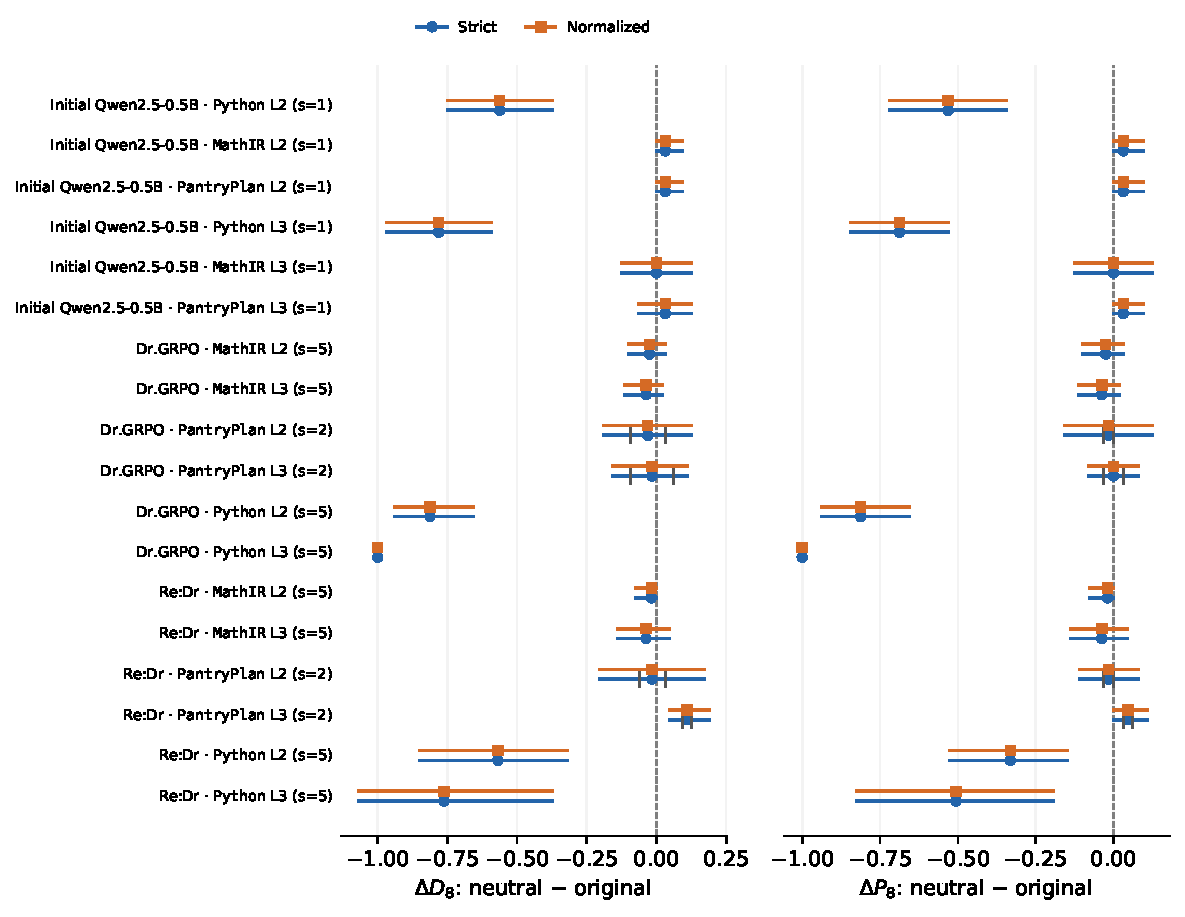
\includegraphics[width=\linewidth]{figures/modebench_prompt_ablation_local.pdf}

\caption{\textbf{\texttt{Python} guidance removal produces the largest wording effects in this panel.} Neutral-minus-original $D_8$ (left) and $P_8$ (right) for the initial Qwen2.5-0.5B checkpoint and Level-2-trained Dr.GRPO and Re:Dr on \texttt{Python}, \texttt{MathIR}, and \texttt{PantryPlan} at Levels 2 and 3, with 32 paired problems and eight draws per arm. Blue circles use strict verification; orange squares use formatting normalization. Horizontal bars are pointwise 95\% bootstrap intervals; the vertical dashed line marks zero. Five-seed groups resample training seeds and paired problems; \texttt{PantryPlan} and initial-model intervals condition on two checkpoints and one checkpoint, respectively. Gray marks show the individual effects for the two \texttt{PantryPlan} training seeds. }

\label{fig:prompt-hints-local}

\end{figure}



\begin{samepage}
\paragraph{Two-seed \texttt{PantryPlan} effects.} Intervals condition on the two checkpoints and do not quantify training-seed variability. The effects for each seed are shown below; each pair gives $(\Delta P_8,\Delta D_8)$.
\begin{center}\small
\begin{tabular}{llcc}
\toprule
Method & Level & First seed & Second seed \\
\midrule
Dr.GRPO & 2 & $(+0.000, +0.03)$ & $(-0.031, -0.09)$ \\
Dr.GRPO & 3 & $(+0.031, +0.06)$ & $(-0.031, -0.09)$ \\
Re:Dr & 2 & $(-0.031, -0.06)$ & $(+0.000, +0.03)$ \\
Re:Dr & 3 & $(+0.031, +0.12)$ & $(+0.062, +0.09)$ \\
\bottomrule
\end{tabular}
\end{center}
\end{samepage}